\documentclass[tikz,border=0pt]{standalone}
\usepackage[T1]{fontenc}
\usepackage{helvet}
\renewcommand{\familydefault}{\sfdefault}
% Reuse accepted label-free artwork through vector viewports; no pixel editing.
\usepackage{graphicx}
\usetikzlibrary{arrows.meta,calc}
\tikzset{flow/.style={-{Stealth[length=1.6mm,width=1.1mm]},line width=.75pt},
 wirelabel/.style={fill=white,inner sep=1.2mm},
 every node/.style={font=\fontsize{9}{11}\selectfont,align=center,inner sep=1pt}}
% Arguments: source left/top/right/bottom pixels; destination left/bottom/width mm.
\newcommand{\artpiece}[7]{
 \pgfmathsetmacro{\pieceScale}{#7/((#3-#1)*.1)}
 \begin{scope}[shift={(#5,#6)},scale=\pieceScale,transform shape]
  \clip (0,0) rectangle ({(#3-#1)*.1},{(#4-#2)*.1});
  \node[anchor=south west,inner sep=0pt] at ({-#1*.1},{-(931-#4)*.1})
   {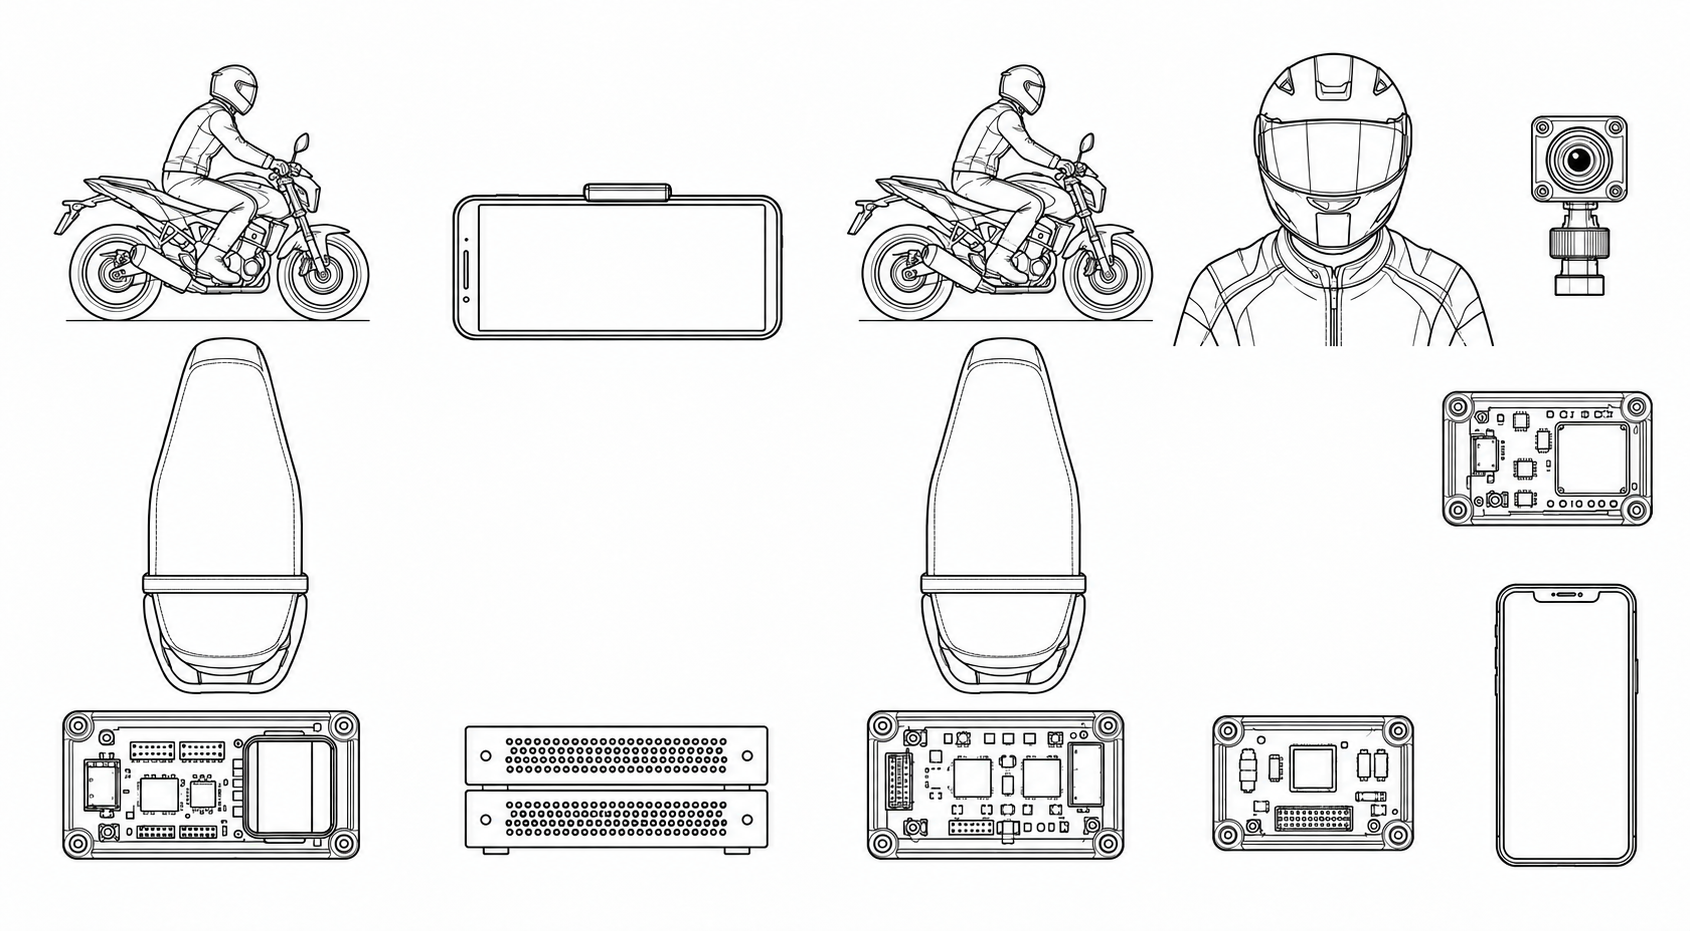
\includegraphics[width=169mm]{artwork-original.png}};
 \end{scope}}
\newcommand{\marker}[2]{
 \fill[white] (#1-2.4,#2-2.4) rectangle (#1+2.4,#2+2.4);
 \fill (#1-2,#2-2) rectangle (#1+2,#2+2);
 \fill[white] (#1-1.2,#2-1.2) rectangle (#1+1.2,#2+1.2);
 \fill (#1-1.2,#2-1.2) rectangle (#1,#2);
 \fill (#1,#2) rectangle (#1+1.2,#2+1.2);
}
\newcommand{\phoneglyph}[2]{
 \begin{scope}[shift={(#1,#2)}]
  \draw[densely dotted] (-8,0)--(8,0) (0,-13)--(0,13);
  \draw (0,10) .. controls (7,12) and (3,4) .. (7,-1)
    .. controls (11,-9) and (-4,-13) .. (-6,-7)
    .. controls (-9,0) and (-6,8) .. (0,10);
 \end{scope}}

\usetikzlibrary{patterns}
\tikzset{frameone/.style={line width=1.5pt,line join=miter,line cap=butt},frametwo/.style={line width=1pt,line join=miter,line cap=butt}}
\begin{document}
\begin{tikzpicture}[x=1mm,y=1mm,line width=.65pt,line cap=round,line join=miter]
\path[use as bounding box] (0,0) rectangle (240,180);

\draw[frameone] (3,66) rectangle (74,177) (78,66) rectangle (145,177) (149,66) rectangle (237,177);
\node at (41,172) {A. Sense the commute};
\node at (111.5,172) {B. Read and transmit};
\node at (190.5,172) {C. Glance and retrieve};
\artpiece{35}{48}{380}{328}{14}{117}{54}
\artpiece{130}{330}{315}{700}{32}{72}{18}
\foreach \xx in {38.2,44}{\draw[fill=white] (\xx-1,87.7) rectangle (\xx+1,89.7);}
\node[align=center] at (41,111) {2 force-sensitive resistors\\under the seat};
\artpiece{55}{708}{370}{865}{89}{132}{45}
\node at (111.5,125) {Genuino microcontroller};
\draw[flow] (50,90)--(84,90)--(84,142)--(89,142);
\node[align=center] at (111.5,111) {Read two channels\\and add timestamps};
\draw[frametwo] (88,78) rectangle (135,99);
\draw (91,84)--(96,84)--(96,94)--(100,94)--(100,88)--(106,88);
\draw[dashed] (110,84)--(115,84)--(115,90)--(120,90)--(120,95)--(131,95);
\node at (111.5,72) {0--1023 sensor readings};
\artpiece{445}{178}{790}{345}{158}{120}{65}
\draw (165,133)--(170,133)--(170,141)--(175,141)--(175,129)--(180,129)--(180,136)--(188,136);
\draw (207,135) circle (6);\draw (207,141)--(207,135)--(212,132);
\node[align=center] at (190.5,160) {Past 3 minutes / whole ride\\pressure variation and duration};
\draw[flow] (134,143)--(158,143);
\artpiece{455}{720}{775}{860}{171.5}{74}{38}
\draw[flow] (190.5,120)--(190.5,91);
\node[anchor=west] at (195,105) {Mobile internet};
\node at (190.5,70) {Remote storage and retrieval};
% Labels after all connectors; a crossing label masks the line underneath.
\node[wirelabel] at (111.5,159) {Bluetooth Low Energy};
\draw[frameone] (3,23) rectangle (237,62);
\node[anchor=west] at (7,57) {D. Four equal bins of pressure readings: how dashboard marks are encoded};
\foreach \xx/\lo/\hi/\pat in {16/0/255/north east lines,70/256/511/north west lines,124/512/767/crosshatch,178/768/1023/dots}{
 \draw[pattern=\pat,pattern color=black] (\xx,37) rectangle (\xx+46,49);
 \node at (\xx+23,32) {\lo--\hi};
}
\node at (120,26.5) {Schematic pattern key for pressure bins; these are not posture classes};
\draw[frameone] (3,3) rectangle (237,19);
\node[anchor=west,align=left] at (7,11) {Implemented demonstration.\\Supports reflection; health benefits were not evaluated.};
\node[anchor=east,align=right] at (233,11) {Bagalkot and colleagues (2017), 420--423.\\Human--Computer Interaction: INTERACT; source: 421--422.\\Artwork: conceptual reconstruction; traces are illustrative.};
\end{tikzpicture}
\end{document}
